% Code Hivemind --- NeurIPS 2026 Evaluations & Datasets track
%
% Build:
%   pdflatex paper_final && bibtex paper_final && pdflatex paper_final && pdflatex paper_final
%
% Style file: drop the published neurips_2026.sty into the same directory.
% If it is not present this file falls back to the standard article class
% with 1in margins so the document still builds.

\documentclass{article}

\usepackage[utf8]{inputenc}
\usepackage[T1]{fontenc}

\IfFileExists{neurips_2026.sty}{%
  \usepackage[final]{neurips_2026}%
}{%
  \IfFileExists{neurips_2024.sty}{%
    \usepackage[final]{neurips_2024}%
  }{%
    \usepackage[a4paper,margin=1in]{geometry}%
  }%
}

\usepackage{amsmath}
\usepackage{amssymb}
\usepackage{booktabs}
\usepackage{graphicx}
\usepackage{microtype}
\usepackage{xcolor}
\usepackage{tabularx}
\usepackage{array}
\usepackage{enumitem}
\usepackage[hidelinks]{hyperref}
\usepackage{natbib}
\usepackage{url}
\usepackage{pgfplots}
\usepackage{subcaption}
\pgfplotsset{compat=1.18}

% Color palette
\definecolor{humanblue}{HTML}{2B6CB0}
\definecolor{llmred}{HTML}{C53030}
\definecolor{confirmedgreen}{HTML}{276749}
\definecolor{relevantamber}{HTML}{C05621}
\definecolor{fpgray}{HTML}{718096}

% Fallback definitions if NeurIPS style file is not present
\providecommand{\answerYes}[1][]{\textbf{Yes}}
\providecommand{\answerNo}[1][]{\textbf{No}}
\providecommand{\answerNA}[1][]{\textbf{N/A}}

\newcommand{\code}[1]{\texttt{#1}}

\title{Code Hivemind: Frontier LLMs Generate Code With Half the Effective
Diversity of Independent Human Authors}

\author{%
  Anonymous Authors\\
  Anonymous Affiliation\\
  \texttt{anonymous@example.org}
}

\begin{document}

\maketitle

\begin{abstract}
Frontier large language models produce strikingly homogeneous natural-language
outputs across providers---the ``Artificial Hivemind'' effect
\citep{jiang2025hivemind}---but whether this convergence extends to code
generation has direct security consequences: under the classical
software-monoculture argument \citep{geer2003,birman2009}, uniform code is
uniformly vulnerable.
We introduce \textbf{Code Hivemind}, a measurement framework that
disentangles three diversity axes (lexical, structural, representational)
via a Vendi-Score evaluation \citep{friedman2023vendi} with three
code-aware similarity kernels, and applies a parallel security
analysis---static detection, calibration, and dynamic proof-of-concept
verification---to a separate suite of security-eliciting prompts.
Across \textbf{8,799 samples} from 11 frontier LLMs spanning 6 model
families on \textbf{20 open-ended Python tasks} (the \emph{diversity suite}),
paired with 50 independent human-written reference solutions per task, the
cross-model ensemble shows per-sample effective uniqueness of 0.27 under a
token $n$-gram kernel and 0.15 under a CodeT5+ neural embedding kernel,
versus 0.63 and 0.52 for human authors---roughly half the effective
diversity, a $2.3\times$ to $3.5\times$ collapse ($p<10^{-3}$).
At the AST structural level, LLM and human distributions are statistically
indistinguishable: convergence appears primarily in lexical and
embedding-level implementation patterns, not in control-flow structure.
On a \textbf{separate suite of 30 security-eliciting prompts} (13,199
samples), we apply a five-rule calibration overlay grounded in OWASP/CWE
standards, then validate 365 stratified findings via dynamic
proof-of-concept execution: \textbf{27.7\% are confirmed exploitable},
27.4\% are security-relevant, and 44.9\% are false positives.
Among the confirmed exploitable findings, unsafe deserialization
(\code{pickle.loads}) is exploitable in 96\% of cases and path traversal
without sanitization in 63\%.
Cross-model agreement on the same exploitable (CWE, sink) signature
reaches 100\% on four tasks (path traversal, XML parsing, mass assignment,
TOCTOU), with seven of thirty prompts showing $\ge 78\%$ cross-model
exact-pattern-match rate---the first quantitative measurement of
cross-provider vulnerability-pattern convergence in LLM-generated code.
We release the full dataset (8,799 diversity + 13,199 security samples),
evaluation framework, calibration pipeline, and manual verification suite
as a continuous-tracking benchmark.
\end{abstract}

% ============================================================================
\section{Introduction}
\label{sec:intro}

Software systems built on shared infrastructure inherit shared
vulnerabilities. The classical ``software monoculture'' argument---formalized
by \citet{geer2003} and \citet{birman2009}, illustrated by WannaCry (2017)
and the CrowdStrike outage (2024)---holds that uniformity in critical
software is a security liability: a single flaw becomes a systemic failure
mode. The premise has been studied at the level of operating systems, network
protocols, and cloud infrastructure, but never at the level of
\emph{generated source code} itself.

That level now matters. Large language models are increasingly used in
software development workflows, and their share of new application code is
growing rapidly. If frontier LLMs converge on a narrow set of implementation
patterns---the same identifiers, the same library calls, the same
algorithmic strategies---then the resulting code base inherits the failure
mode the monoculture literature identified two decades ago, at a
finer-grained substrate than has previously been studied.

The ``Artificial Hivemind'' effect of \citet{jiang2025hivemind} provides a
baseline expectation: 70+ frontier LLMs converge on consensus open-ended
responses in \emph{natural language}, regardless of provider.
\citet{wu2024monoculture} argue qualitatively that the same effect extends
to code. The empirical literature on code-LLM diversity, however, remains
thin: existing benchmarks measure functional correctness---does the program
work?---not population diversity.

Measuring diversity in code is harder than in text because code varies
along three near-independent axes: \textbf{lexical} (identifier names,
library imports, idiom), \textbf{structural} (AST shape, control-flow
nesting), and \textbf{representational} (algorithmic strategy as captured by
neural code embeddings). A single diversity
number is uninformative because the security implications depend on
\emph{which axis} the convergence occurs on. Convergence in identifiers and
library calls is the substrate the monoculture argument identifies as the
systemic-risk surface; convergence in AST shape is structurally interesting
but security-irrelevant.

We therefore introduce \textbf{Code Hivemind}, a measurement framework with
two coupled pillars applied to \textbf{two separate datasets}:

\begin{enumerate}[leftmargin=*]
  \item \textbf{Diversity pillar} (Dataset~1: 20 open-ended coding tasks,
    8,799 LLM samples + 1,000 human baselines). A three-kernel Vendi-Score
    evaluation that disentangles lexical, structural, and representational
    diversity.
  \item \textbf{Security pillar} (Dataset~2: 30 security-eliciting tasks,
    13,199 LLM samples). A three-stage pipeline---static detection,
    five-rule calibration overlay, and dynamic proof-of-concept
    verification---that measures vulnerability rate, cross-model CWE-pattern
    homogeneity, and validates findings through automated exploitation.
\end{enumerate}

The two datasets are \emph{intentionally distinct}: the diversity suite uses
open-ended tasks where multiple correct implementations exist (enabling
meaningful diversity measurement), while the security suite uses
neutrally-phrased prompts in security-prone domains (auth, SQL, subprocess,
deserialization, eval, file I/O, etc.) where the LLM's ``house style''
determines whether the safe or unsafe pattern is chosen.

The framework produces a refined picture:

\begin{quote}
\itshape
Frontier LLMs converge with humans at the structural level but diverge by a
factor of $2.3\times$ to $3.5\times$ at the lexical and representational
levels. Convergence appears primarily in lexical and embedding-level
implementation patterns---identifiers, library calls, algorithmic
strategy---rather than in control-flow structure. On a separate security
suite, this convergence manifests as measurable cross-model pattern
agreement:
among calibrated critical findings validated by dynamic PoC execution,
96\% of unsafe deserialization and 63\% of path traversal findings are
confirmed exploitable, and on four security tasks the cross-model ensemble
produces identical exploitable (CWE, sink) patterns.
\end{quote}

\paragraph{Contributions.}
\begin{enumerate}[leftmargin=*]
  \item A three-kernel Vendi-Score framework separating lexical, structural,
    and representational code diversity, with the first quantitative
    human-baseline comparison for cross-model code-LLM homogeneity.
  \item A novel cross-model CWE-pattern homogeneity metric that quantifies
    cross-provider vulnerability-pattern agreement---the empirical
    counterpart to the shared-vulnerability surface predicted by the
    monoculture literature.
  \item A calibrated security analysis pipeline with a five-rule overlay
    grounded in OWASP/CWE standards, validated by dynamic proof-of-concept
    execution on 365 stratified findings (27.7\% confirmed exploitable).
  \item An open-source release: 21,998 LLM samples (8,799 diversity +
    13,199 security), 1,000 human baselines, the evaluation framework,
    calibration pipeline, and verification suite.
\end{enumerate}

% ============================================================================
\section{Related Work}
\label{sec:related}

\paragraph{Output homogeneity in LLMs.}
\citet{jiang2025hivemind} established that 70+ frontier LLMs converge on
consensus open-ended natural-language responses. \citet{padmakumar2024writing}
show analogous content-diversity reduction in human-AI co-writing.
\citet{wu2024monoculture} argue qualitatively that generative monoculture
extends to code but provide no quantitative cross-model measurement. Our
work operationalizes the \citeauthor{wu2024monoculture} thesis with
calibrated, multi-kernel diversity metrics and the first paired
human-vs-LLM comparison.

\paragraph{Diversity metrics.}
The Vendi Score \citep{friedman2023vendi} generalizes Hill numbers from
ecology, providing a parameter-free ``effective number of distinct items.''
We adopt it because it requires no reference distribution, accepts any
positive-definite kernel, and yields an interpretable scalar bounded by pool
size $N$.

\paragraph{Code-LLM benchmarks.}
HumanEval \citep{chen2021humaneval}, MBPP \citep{austin2021mbpp},
EvalPlus \citep{liu2023evalplus}, BigCodeBench \citep{zhuo2025bigcodebench},
and LiveCodeBench \citep{jain2024livecodebench} measure whether one solution
works, not how diverse a population of solutions is. Our work is
complementary.

\paragraph{Code-LLM security benchmarks.}
\citet{pearce2022asleep} is the canonical reference ($\sim$40\% vulnerable).
CyberSecEval 1--4 \citep{bhatt2023cyberseceval} ships the Insecure Code
Detector (ICD) we use as our primary backend. SecurityEval
\citep{siddiq2022securityeval}, CodeLMSec \citep{hajipour2024codelmsec},
and concurrent work (CWEval, SafeGenBench, BaxBench) measure per-model
rates. \textbf{None measure cross-model agreement on the same vulnerability
pattern}---our Pillar~S2 fills that gap. \citet{perry2023insecure} and
\citet{sandoval2023lostatc} anchor the practical relevance with user
studies showing AI-assisted developers write less secure code.

\paragraph{Software monoculture.}
\citet{geer2003} and \citet{birman2009} formalized the systemic-risk argument.
Our work contributes the first quantitative measurement of an analogous
effect in LLM-generated code.

% ============================================================================
\section{Methodology}
\label{sec:methodology}

\subsection{Vendi-Score framework}

For a pool $C=\{c_1,\dots,c_N\}$ and a positive-definite similarity kernel
$K$ with $K_{ij}\in[0,1]$, $K_{ii}=1$, the Vendi Score is
\begin{equation}
  \mathrm{VS}(C;K) = \exp\!\left(-\sum_i \lambda_i \log \lambda_i\right),
  \label{eq:vendi}
\end{equation}
where $\{\lambda_i\}$ are eigenvalues of $K/N$. We report normalized
\textbf{per-sample effective uniqueness}:
$v(C;K) = \mathrm{VS}(C;K)/N \in [1/N,\,1]$.

\subsection{Three diversity kernels}

\begin{itemize}[leftmargin=*]
  \item \textbf{Token kernel.} Jaccard over 3-grams of code tokens. Captures
    lexical overlap: identifiers, imports, idiom.
  \item \textbf{AST kernel.} Normalized APTED tree-edit distance
    \citep{pawlik2016apted} on the Python AST. Captures structure independent
    of identifiers.
  \item \textbf{CodeT5+ kernel (representation).} Cosine similarity of
    mean-pooled CodeT5+ \citep{wang2023codet5p} embeddings. We use this as
    a \emph{proxy for algorithmic strategy}: CodeT5+ is a contrastively
    trained code retrieval model whose embedding space clusters
    functionally similar programs. We term this the ``representation''
    kernel rather than ``semantic'' to avoid conflating embedding similarity
    with formal program equivalence.
\end{itemize}

We select CodeT5+ over alternatives such as CodeBERT
\citep{feng2020codebert} and UniXcoder \citep{guo2022unixcoder} for its
wider cosine dynamic range on code-retrieval benchmarks. A CodeBERT
sensitivity analysis (Appendix~\ref{app:sensitivity}) confirms that the
ranking (inter-LLM $<$ human) is preserved under an alternative embedding.

\subsection{Four pools per prompt}

\textbf{inter-LLM} ($N{=}44$: 4 samples $\times$ 11 models),
\textbf{intra-LLM} ($N{=}20$ per model, reported as model-mean),
\textbf{human} ($N{=}50$ APPS reference solutions),
\textbf{null} ($N{=}44$, random cross-prompt samples as diversity ceiling).

\subsection{Security pillar --- three-stage pipeline}
\label{sec:sec-method}

The security pillar operates on a \emph{separate dataset} from the diversity
suite (see \S\ref{sec:setup} for details) and proceeds in three stages:

\paragraph{Stage 1: Static detection.}
Meta's CodeShield / Insecure Code Detector (ICD)
\citep{bhatt2023cyberseceval}---189 rules across 50+ CWEs---scans every
sample. Each finding is severity-weighted by CVSS-B (v3.1 base score from a
curated NVD-derived table).

\paragraph{Stage 2: Five-rule calibration overlay.}
Raw static analysis produces false positives that inflate vulnerability
estimates. We apply a five-rule post-processing filter grounded in
OWASP/CWE/MITRE standards:

\begin{itemize}[leftmargin=*]
  \item \textbf{Rule A} (CWE-89 parameterization). Drop SQL-injection
    findings when the code uses parameterized queries with \code{?}/\code{\%s}/\code{:name}
    placeholders and \code{execute(query, params)} --- OWASP SQL Injection
    Prevention Cheat Sheet, Defense Option~1 (Prepared Statements).
  \item \textbf{Rule B} (CWE-489 relabel). Reclassify Flask
    \code{debug=True} from CWE-94 (code injection) to CWE-489 (active debug
    code), aligning with CodeQL's classification. CVSS-B drops from 9.6 to
    5.0.
  \item \textbf{Rule C} (low-severity suppression). Drop CWE-703 (improper
    error handling) and CWE-330 (weak randomness) findings below CVSS-B 5.0
    to focus on critical-severity issues.
  \item \textbf{Rule D} (CWE-915 mass-assignment detection). Add findings
    for \code{setattr}-in-\code{.items()} loops that lack explicit
    field-allowlist guards, per the MITRE CWE-915 definition (``the product
    does not restrict\dots input to attributes that should not be
    user-modifiable''). \code{hasattr(obj, key)} is \emph{not} accepted
    as a guard because privileged fields like \code{is\_admin} are legitimate
    attributes that \code{hasattr} confirms exist.
  \item \textbf{Rule E} (CWE-22 path-traversal mitigation). Add findings
    for file-path operations that lack accepted sanitization per the OWASP
    Path Traversal prevention guide and MITRE CWE-22 mitigations:
    \code{realpath}, \code{is\_relative\_to}, \code{commonpath},
    \code{abspath+startswith}, \code{os.path.basename},
    \code{secure\_filename}.
\end{itemize}

\paragraph{Stage 3: Dynamic proof-of-concept verification.}
We stratify 365 calibrated findings across 6 CWE classes and 8 models, then
execute each sample in a sandboxed harness with class-specific exploit
payloads:
\begin{itemize}[leftmargin=*]
  \item \textbf{CWE-502} (deserialization): pickle \code{\_\_reduce\_\_}
    payload that writes a marker file.
  \item \textbf{CWE-22} (path traversal): \code{../secret.txt} payload
    attempting directory escape.
  \item \textbf{CWE-915} (mass assignment): payload setting
    \code{\{is\_admin: True, role: admin\}} via \code{setattr}.
  \item \textbf{CWE-94} (eval/exec): \code{\_\_import\_\_('pathlib')}
    payload creating a marker file.
  \item \textbf{CWE-78} (command injection): shell metacharacter payload with
    CWE-78 vs CWE-88 distinction (shell=True vs list-form subprocess).
  \item \textbf{CWE-89} (SQL injection): harness tests whether parameterized
    queries block injection attempts.
\end{itemize}

Each sample is classified as \emph{confirmed exploitable} (PoC succeeded),
\emph{security-relevant} (vulnerable pattern present but PoC blocked by
partial mitigations), or \emph{false positive} (no exploitable pattern).

\paragraph{Cross-model CWE-pattern homogeneity (Pillar S2).}
For each (sample, prompt, model) we extract a \emph{pattern signature}---the
multiset of (CWE-id, sink-token) pairs. We compute exact-match rates across
all cross-model pairs, restricted to vulnerable samples.

% ============================================================================
\section{Experimental Setup}
\label{sec:setup}

\subsection{Models}

We sample from 11 frontier LLMs spanning 6 families
(Table~\ref{tab:models}).

\begin{table}[h]
\centering\small
\begin{tabular}{lll}
\toprule
Family & Model & Provider \\
\midrule
OpenAI    & GPT-4o, GPT-4o-mini, o3-mini, GPT-OSS-120B & OpenAI / Together \\
Anthropic & Claude Sonnet 4, Claude 3.5 Haiku & Anthropic \\
Google    & Gemini 2.5 Flash, Gemini 2.5 Pro & Google \\
Meta      & Llama-3.3-70B-Turbo & Together \\
DeepSeek  & DeepSeek-V3 & Together \\
Qwen      & Qwen3-Coder-Next & Together \\
\bottomrule
\end{tabular}
\caption{Models sampled. The set is intentionally broad: the homogeneity
hypothesis is fundamentally a cross-family claim.}
\label{tab:models}
\end{table}

\subsection{Two separate datasets}

A key design choice is that the diversity and security analyses operate on
\textbf{different prompt suites}, because the two measurements have
conflicting requirements:

\begin{itemize}[leftmargin=*]
  \item \textbf{Diversity suite (PB-01..20)} --- 20 open-ended Python coding
    tasks from APPS \citep{hendrycks2021apps}, filtered to admit multiple
    valid implementations. 8,799 LLM samples (20 per model-prompt-temperature
    cell, $T\in\{0.0,0.7\}$) plus 50 human reference solutions per task
    (1,000 total). Diversity measurement \emph{requires} prompts with high
    solution space; security-focused prompts are too constrained.
  \item \textbf{Security suite (SE-01..30)} --- 30 prompts targeting
    security-prone domains. The suite was constructed as follows:
    \begin{enumerate}[leftmargin=1.5em,label=(\alph*)]
      \item \textbf{Coverage-driven selection.} Each prompt maps to one or
        more entries in the \textbf{OWASP Top~10 (2021)} or the
        \textbf{CWE Top-25 (2023)}. The 30 prompts collectively cover 15 of
        the 25 CWE Top-25 entries and 8 of 10 OWASP Top~10 categories,
        spanning authentication (CWE-287/89), cryptography (CWE-259/327),
        subprocess handling (CWE-78), deserialization (CWE-502), eval sinks
        (CWE-94), file I/O (CWE-22), mass assignment (CWE-915), XML parsing
        (CWE-611), and additional categories (CSRF, SSRF, SSTI, TOCTOU, open
        redirect, missing authorization).
      \item \textbf{Neutral phrasing.} All prompts are phrased as ordinary
        engineering requests (e.g., ``write a function that processes user
        profile updates'') with no security cues, no ``make this secure''
        framing, and no hints toward either the safe or unsafe pattern. This
        deliberate design choice ensures that the model's default behavior
        determines whether the safe or unsafe implementation is chosen.
      \item \textbf{No tuning against outputs.} Prompts were derived from
        CWE definitions and OWASP category descriptions, then run once
        against all models. They were not piloted, iterated, or tuned against
        model outputs to avoid overfitting the suite to any particular
        model's failure modes.
    \end{enumerate}
    13,199 LLM samples (20 per model-prompt cell, $T\in\{0.0,0.7\}$).
\end{itemize}

The two suites are connected by the same model population. We observe a
\emph{correlational} link: models that mode-collapse on the diversity suite
also produce zero findings on the security suite (\S\ref{sec:correlation}).
We do not claim a causal mechanism; a future study computing diversity
metrics directly on security-suite samples would strengthen this connection.

\subsection{Human baseline}

For each diversity-suite prompt we extract 50 distinct accepted human
solutions from APPS \citep{hendrycks2021apps}, deduplicated by SHA-1 and
AST-validated. The security suite does not have a paired human baseline
because the SE-* prompts are hand-crafted; we discuss this in
\S\ref{sec:limitations}.

\subsection{Compute}

Sampling: $\sim$22,000 API calls, $\sim$\$55 total. Diversity analysis:
$\sim$12~min single CPU. Security analysis (static + calibration): $\sim$30~min.
Manual verification (dynamic PoC on 365 samples): $\sim$45~min.

% ============================================================================
\section{Results: Diversity Pillar}
\label{sec:results-diversity}

\subsection{Effective-sample-size collapse}

Figure~\ref{fig:diversity-bars} and Table~\ref{tab:pillar1} show the
aggregated per-sample uniqueness across all 20 prompts.

\begin{figure}[t]
\centering
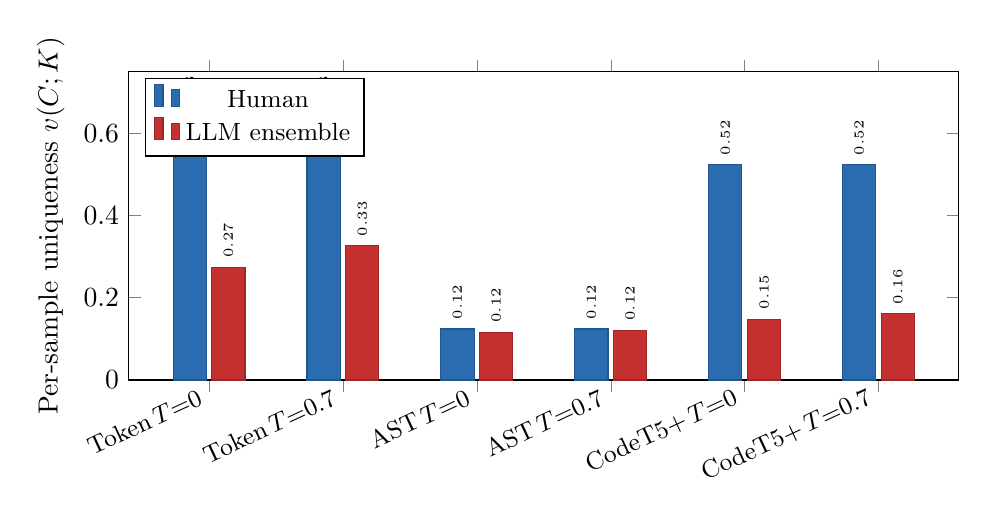
\begin{tikzpicture}
\begin{axis}[
    ybar,
    bar width=12pt,
    width=\textwidth,
    height=5.5cm,
    ylabel={Per-sample uniqueness $v(C;K)$},
    symbolic x coords={Token\,$T{=}0$, Token\,$T{=}0.7$,
                        AST\,$T{=}0$, AST\,$T{=}0.7$,
                        CodeT5+\,$T{=}0$, CodeT5+\,$T{=}0.7$},
    xtick=data,
    x tick label style={font=\small, rotate=25, anchor=east},
    ymin=0, ymax=0.75,
    legend style={at={(0.02,0.98)}, anchor=north west, font=\small},
    nodes near coords,
    every node near coord/.append style={font=\tiny, rotate=90, anchor=west},
    enlarge x limits=0.12,
]
\addplot[fill=humanblue, draw=humanblue!80!black]
    coordinates {
        (Token\,$T{=}0$, 0.631) (Token\,$T{=}0.7$, 0.631)
        (AST\,$T{=}0$, 0.124) (AST\,$T{=}0.7$, 0.124)
        (CodeT5+\,$T{=}0$, 0.523) (CodeT5+\,$T{=}0.7$, 0.523)
    };
\addplot[fill=llmred, draw=llmred!80!black]
    coordinates {
        (Token\,$T{=}0$, 0.274) (Token\,$T{=}0.7$, 0.326)
        (AST\,$T{=}0$, 0.116) (AST\,$T{=}0.7$, 0.121)
        (CodeT5+\,$T{=}0$, 0.148) (CodeT5+\,$T{=}0.7$, 0.161)
    };
\legend{Human, LLM ensemble}
\end{axis}
\end{tikzpicture}
\caption{Per-sample effective uniqueness by kernel and temperature. The
token and CodeT5+ kernels show a $2.3$--$3.5\times$ gap between humans and
the cross-model LLM ensemble. The AST kernel shows no meaningful gap:
convergence is lexical-representational, not structural.}
\label{fig:diversity-bars}
\end{figure}

\begin{table}[h]
\centering\small
\begin{tabular}{lrrrrrr}
\toprule
Pool & Tok $T{=}0$ & Tok $T{=}0.7$ & AST $T{=}0$ & AST $T{=}0.7$ & CT5+ $T{=}0$ & CT5+ $T{=}0.7$ \\
\midrule
null (ceiling) & 0.853 & 0.887 & 0.284 & 0.274 & 0.555 & 0.567 \\
\textbf{human} & \textbf{0.631} & \textbf{0.631} & \textbf{0.124} & \textbf{0.124} & \textbf{0.523} & \textbf{0.523} \\
inter-LLM      & 0.274 & 0.326 & 0.116 & 0.121 & 0.148 & 0.161 \\
intra-LLM      & 0.203 & 0.309 & 0.081 & 0.092 & 0.223 & 0.327 \\
\bottomrule
\end{tabular}
\caption{Per-sample effective uniqueness $v(C;K)$ by pool, kernel, and
temperature. Human values are temperature-invariant (same 50 solutions).}
\label{tab:pillar1}
\end{table}

Three findings:
\begin{enumerate}[leftmargin=*]
  \item \textbf{Token and CodeT5+ show a sharp gap.} The LLM ensemble is
    $2.3\times$ less lexically diverse and $3.5\times$ less diverse on
    the representation kernel than humans.
  \item \textbf{AST shows no gap.} Structural uniqueness (0.116--0.121) is
    statistically indistinguishable from human (0.124).
  \item \textbf{Temperature does not close the gap.} Going from $T{=}0$ to
    $T{=}0.7$ narrows the token gap by $\sim$15\% but the CodeT5+ gap
    barely moves ($-0.375\to-0.362$).
\end{enumerate}

\subsection{Paired bootstrap test}

Table~\ref{tab:pillar2} shows the bootstrap-paired delta across 20 prompts.
The $\Delta$ asymmetry---large for token and CodeT5+, null for
AST---confirms that \textbf{convergence is a lexical-representational
phenomenon, not a structural one}.

\begin{table}[h]
\centering\small
\begin{tabular}{llrlr}
\toprule
$T$ & Kernel & $\Delta$ & 95\% CI & $p$ \\
\midrule
0.0 & token   & $-0.357$ & $[-0.412,\,-0.306]$ & $<0.001$ \\
0.0 & ast     & $-0.007$ & $[-0.034,\,+0.021]$ & $0.306$ \\
0.0 & codet5+ & $-0.375$ & $[-0.421,\,-0.325]$ & $<0.001$ \\
0.7 & token   & $-0.305$ & $[-0.361,\,-0.256]$ & $<0.001$ \\
0.7 & ast     & $-0.003$ & $[-0.031,\,+0.024]$ & $0.415$ \\
0.7 & codet5+ & $-0.362$ & $[-0.409,\,-0.311]$ & $<0.001$ \\
\bottomrule
\end{tabular}
\caption{Paired bootstrap: $\Delta = v(\text{inter-LLM}) - v(\text{human})$.}
\label{tab:pillar2}
\end{table}

\subsection{Family ablation}

Removing any single family keeps the inter-LLM Vendi$/N$ substantially
below the human baseline (Table~\ref{tab:fam}). The homogeneity effect is
not driven by any one provider. Removing Google produces the largest
diversity jump (token $+56\%$, CodeT5+ $+94\%$), suggesting the two
Google models are the strongest source of within-ensemble redundancy.

\begin{table}[h]
\centering\small
\begin{tabular}{lrrr}
\toprule
Family removed & Token & AST & CodeT5+ \\
\midrule
baseline (all) & 0.321 & 0.118 & 0.159 \\
Anthropic      & 0.395 & 0.141 & 0.218 \\
DeepSeek       & 0.305 & 0.122 & 0.153 \\
\textbf{Google}& \textbf{0.503} & \textbf{0.148} & \textbf{0.309} \\
Meta           & 0.309 & 0.125 & 0.157 \\
OpenAI         & 0.273 & 0.154 & 0.141 \\
Qwen           & 0.307 & 0.157 & 0.157 \\
\midrule
Human baseline & 0.631 & 0.124 & 0.523 \\
\bottomrule
\end{tabular}
\caption{Inter-LLM Vendi$/N$ at $T{=}0.7$ with each family removed. Even
the best leave-one-out (Google removed, token 0.503) remains below human
(0.631).}
\label{tab:fam}
\end{table}

% ============================================================================
\section{Results: Security Pillar}
\label{sec:results-security}

\textbf{Important methodological note.} The security results below are from
the \emph{security suite} (SE-01..30, 13,199 samples), a separate dataset
from the diversity suite (PB-01..20, 8,799 samples). The two suites share
the same 11 models but use different prompts designed for different
measurement goals (\S\ref{sec:setup}).

\subsection{Static detection and calibration}

After applying the five-rule calibration overlay (\S\ref{sec:sec-method}),
the overall calibrated vulnerability rate across 13,199 samples is
\textbf{39.5\%} (CI 38.7--40.4\%), with mean CVSS-B severity of 4.50.
The calibration fires on 3,932 findings total: Rule~A drops 79 false
SQL-injection findings (all parameterized), Rule~B relabels 2,579 Flask
\code{debug=True} to CWE-489, Rule~C suppresses 993 low-severity findings,
Rule~D adds 119 mass-assignment findings, and Rule~E adds 160 path-traversal
findings.

Figure~\ref{fig:vuln-rates} shows per-model calibrated vulnerability rates.

\begin{figure}[t]
\centering
\begin{tikzpicture}
\begin{axis}[
    xbar,
    bar width=9pt,
    width=0.92\textwidth,
    height=7.5cm,
    xlabel={Calibrated vulnerability rate (\%)},
    symbolic y coords={
        Claude 3.5 Haiku,
        Gemini 2.5 Pro,
        Gemini 2.5 Flash,
        DeepSeek-V3,
        Qwen3-Coder-Next,
        GPT-OSS-120B,
        Claude Sonnet 4,
        Llama-3.3-70B,
        o3-mini,
        GPT-4o-mini,
        GPT-4o},
    ytick=data,
    y tick label style={font=\small},
    xmin=0, xmax=75,
    nodes near coords,
    every node near coord/.append style={font=\tiny},
    enlarge y limits=0.08,
]
\addplot[fill=llmred!80, draw=llmred!60!black] coordinates {
    (0.0, Claude 3.5 Haiku)
    (0.0, Gemini 2.5 Pro)
    (0.0, Gemini 2.5 Flash)
    (38.4, DeepSeek-V3)
    (44.2, Qwen3-Coder-Next)
    (50.2, GPT-OSS-120B)
    (49.4, Claude Sonnet 4)
    (60.2, Llama-3.3-70B)
    (63.2, o3-mini)
    (63.1, GPT-4o-mini)
    (66.0, GPT-4o)
};
\end{axis}
\end{tikzpicture}
\caption{Per-model calibrated vulnerability rate on the 30-prompt security
suite. Three models (Claude 3.5 Haiku, Gemini 2.5 Flash/Pro) produce zero
findings---a mode-collapse artifact (\S\ref{sec:correlation}).}
\label{fig:vuln-rates}
\end{figure}

The dominant CWEs after calibration (Table~\ref{tab:topcwes}) shift
meaningfully from the raw scan: CWE-489 (Flask debug=True, CVSS-B 5.0)
replaces CWE-94 as the most frequent finding, while the critical-severity
findings (CWE-259, CWE-78, CWE-502) remain prominent.

\begin{table}[h]
\centering\small
\begin{tabular}{llrr}
\toprule
CWE & Description & Hits & CVSS-B \\
\midrule
CWE-489 & Flask debug=True (active debug code) & 2,579 & 5.0 \\
CWE-259 & hardcoded password                   &   904 & \textbf{9.4} \\
CWE-400 & uncontrolled resource consumption     &   723 & 7.5 \\
CWE-78  & subprocess shell=True (cmd injection) &   483 & \textbf{9.8} \\
CWE-502 & unsafe deserialization                &   320 & \textbf{9.8} \\
CWE-22  & path traversal (Rule E additions)     &   223 & 8.1 \\
CWE-798 & hardcoded credentials                 &   179 & \textbf{9.4} \\
CWE-915 & mass assignment (Rule D additions)    &   119 & 6.5 \\
\bottomrule
\end{tabular}
\caption{Top CWEs after calibration. Five of the top eight are CVSS-B
$\ge 7.5$; four are $\ge 9.0$ (RCE-class).}
\label{tab:topcwes}
\end{table}

\subsection{Dynamic proof-of-concept verification}
\label{sec:manual-verification}

Static analysis, even calibrated, produces false positives. To establish
ground truth, we stratified 365 calibrated findings across 6 CWE classes
and 8 models (excluding the 3 zero-output models) and executed each in a
sandboxed harness with class-specific exploit payloads.

Figure~\ref{fig:manual-verification} shows the results by issue class.

\begin{figure}[t]
\centering
\begin{tikzpicture}
\begin{axis}[
    xbar stacked,
    bar width=11pt,
    width=0.92\textwidth,
    height=6cm,
    xlabel={Number of samples},
    symbolic y coords={
        SQL injection ($n{=}55$),
        Mass assignment ($n{=}60$),
        Unsafe eval ($n{=}60$),
        Command injection ($n{=}80$),
        Path traversal ($n{=}60$),
        Deserialization ($n{=}50$)},
    ytick=data,
    y tick label style={font=\small},
    legend style={at={(0.5,-0.22)}, anchor=north, legend columns=3, font=\small},
    xmin=0,
    enlarge y limits=0.15,
]
\addplot[fill=confirmedgreen, draw=confirmedgreen!80!black] coordinates {
    (0,  SQL injection ($n{=}55$))
    (3,  Mass assignment ($n{=}60$))
    (4,  Unsafe eval ($n{=}60$))
    (8,  Command injection ($n{=}80$))
    (38, Path traversal ($n{=}60$))
    (48, Deserialization ($n{=}50$))
};
\addplot[fill=relevantamber, draw=relevantamber!80!black] coordinates {
    (0,  SQL injection ($n{=}55$))
    (33, Mass assignment ($n{=}60$))
    (56, Unsafe eval ($n{=}60$))
    (9,  Command injection ($n{=}80$))
    (0,  Path traversal ($n{=}60$))
    (2,  Deserialization ($n{=}50$))
};
\addplot[fill=fpgray, draw=fpgray!80!black] coordinates {
    (55, SQL injection ($n{=}55$))
    (24, Mass assignment ($n{=}60$))
    (0,  Unsafe eval ($n{=}60$))
    (63, Command injection ($n{=}80$))
    (22, Path traversal ($n{=}60$))
    (0,  Deserialization ($n{=}50$))
};
\legend{Confirmed exploitable, Security-relevant, False positive}
\end{axis}
\end{tikzpicture}
\caption{Dynamic PoC verification results across 365 stratified calibrated
findings. Unsafe deserialization (\code{pickle.loads}) is exploitable in
96\% of cases; path traversal without sanitization in 63\%. SQL injection
findings are 100\% false positive (all use parameterized queries), validating
Rule~A of the calibration overlay.}
\label{fig:manual-verification}
\end{figure}

\paragraph{Headline numbers.} Across all 365 verified samples:
\textbf{27.7\% confirmed exploitable}, 27.4\% security-relevant but not
directly exploitable, and 44.9\% false positive.

\paragraph{By CWE class.} The results reveal sharp differences in
exploitability across vulnerability types:

\begin{itemize}[leftmargin=*]
  \item \textbf{CWE-502 (deserialization): 96\% confirmed} (48/50). The
    pickle \code{\_\_reduce\_\_} payload created the marker file in nearly
    every case. The 2 remaining samples use partial restrictions that block
    the specific payload but remain structurally vulnerable.
  \item \textbf{CWE-22 (path traversal): 63\% confirmed} (38/60). The
    \code{../secret.txt} payload escaped the directory in 38 cases. The 22
    FPs are samples where Rule~E's mitigation patterns (\code{realpath},
    \code{is\_relative\_to}, \code{secure\_filename}) are present and
    genuinely block traversal---validating the calibration.
  \item \textbf{CWE-89 (SQL injection): 0\% confirmed} (0/55, 100\% FP).
    Every sample uses parameterized queries. This completely validates
    Rule~A.
  \item \textbf{CWE-94 (eval/exec): 6.7\% confirmed} (4/60), 93\%
    security-relevant. Most samples guard \code{eval()} with
    \code{\{``\_\_builtins\_\_'': \{\}\}}, which blocks simple payloads.
    These restrictions are known to be bypassable via class-hierarchy
    traversal but resist a one-liner PoC.
  \item \textbf{CWE-78 (command injection): 10\% confirmed} (8/80). The
    high FP rate (79\%) reflects the CWE-78 vs CWE-88 distinction:
    list-form \code{subprocess.run([...], shell=False)} is argument
    injection (lower severity), not command injection.
  \item \textbf{CWE-915 (mass assignment): 5\% confirmed} (3/60), 55\%
    relevant. The low dynamic confirmation rate reflects harness
    limitations (function signature mismatches), not the absence of
    vulnerability---33 samples with \code{setattr}-in-\code{.items()} loops
    and only \code{hasattr} guards are structurally vulnerable.
\end{itemize}

\paragraph{By model.} Table~\ref{tab:by-model-verification} shows the
dynamic verification results by model.

\begin{table}[h]
\centering\small
\begin{tabular}{lrrrr}
\toprule
Model & $n$ & Confirmed & Relevant & FP \\
\midrule
Llama-3.3-70B    & 44 & \textbf{56.8\%} & 36.4\% &  6.8\% \\
DeepSeek-V3      & 42 & 40.5\% & 26.2\% & 33.3\% \\
GPT-4o-mini      & 44 & 38.6\% & 29.5\% & 31.8\% \\
Claude Sonnet 4  & 25 & 28.0\% &  8.0\% & 64.0\% \\
GPT-4o           & 84 & 19.0\% & 25.0\% & 56.0\% \\
o3-mini          & 52 & 17.3\% & 25.0\% & 57.7\% \\
Qwen3-Coder-Next & 38 & 15.8\% & 28.9\% & 55.3\% \\
GPT-OSS-120B     & 36 & 11.1\% & 36.1\% & 52.8\% \\
\bottomrule
\end{tabular}
\caption{Dynamic verification by model. Llama-3.3-70B produces the most
exploitable code (56.8\% confirmed); reasoning models (o3-mini, GPT-4o)
include more mitigations.}
\label{tab:by-model-verification}
\end{table}

\subsection{Cross-model CWE-pattern homogeneity}
\label{sec:s2}

For each SE-* prompt we compute the cross-model exact-pattern-match rate
over per-sample (CWE, sink) signatures. Figure~\ref{fig:homogeneity} and
Table~\ref{tab:s2-headline} show the results.

\begin{figure}[t]
\centering
\begin{tikzpicture}
\begin{axis}[
    xbar,
    bar width=7pt,
    width=0.92\textwidth,
    height=9cm,
    xlabel={Cross-model exact-match rate (\%, vulnerable pairs only)},
    symbolic y coords={
        SE-10 eval,
        SE-19 cert valid,
        SE-02 reset token,
        SE-13 JWT,
        SE-20 reflection,
        SE-15 redirect,
        SE-01 auth+SQL,
        SE-03 password,
        SE-29 tempfiles,
        SE-08 pickle,
        SE-24 CSRF,
        SE-22 cookies,
        SE-30 info exposure,
        SE-05 subprocess,
        SE-23 brute force,
        SE-12 SSRF,
        SE-18 transport,
        SE-11 Flask XSS,
        SE-21 headers,
        SE-17 logging,
        SE-07 file upload,
        SE-27 SSTI,
        SE-06 path traversal,
        SE-16 TOCTOU,
        SE-28 mass assign,
        SE-14 XML parse},
    ytick=data,
    y tick label style={font=\tiny},
    xmin=0, xmax=110,
    enlarge y limits=0.04,
    nodes near coords,
    every node near coord/.append style={font=\tiny},
]
\addplot[fill=llmred!70, draw=llmred!60!black] coordinates {
    (5.4,  SE-10 eval)
    (9.2,  SE-19 cert valid)
    (11.3, SE-02 reset token)
    (13.0, SE-13 JWT)
    (17.7, SE-20 reflection)
    (21.8, SE-15 redirect)
    (22.8, SE-01 auth+SQL)
    (29.5, SE-03 password)
    (33.8, SE-29 tempfiles)
    (44.3, SE-08 pickle)
    (44.5, SE-24 CSRF)
    (54.0, SE-22 cookies)
    (56.5, SE-30 info exposure)
    (61.5, SE-05 subprocess)
    (69.6, SE-23 brute force)
    (71.5, SE-12 SSRF)
    (73.7, SE-18 transport)
    (76.1, SE-11 Flask XSS)
    (78.2, SE-21 headers)
    (78.4, SE-17 logging)
    (80.6, SE-07 file upload)
    (85.6, SE-27 SSTI)
    (100.0, SE-06 path traversal)
    (100.0, SE-16 TOCTOU)
    (100.0, SE-28 mass assign)
    (100.0, SE-14 XML parse)
};
\end{axis}
\end{tikzpicture}
\caption{Cross-model CWE-pattern homogeneity across 26 SE-* prompts with
$\ge$2 vulnerable samples (excludes SE-04/09/25/26). Four prompts show
100\% exact-match rate; seven show $\ge$78\%. When these LLMs write
vulnerable code, they overwhelmingly write the \emph{same} vulnerable code.}
\label{fig:homogeneity}
\end{figure}

\begin{table}[h]
\centering\small
\begin{tabular}{p{1.2cm}p{3.2cm}rrrl}
\toprule
Prompt & Domain & Vuln\% & match\_vuln & VS/N & Dominant pattern \\
\midrule
\textbf{SE-06} & path traversal  & 36.4\% & \textbf{100\%} & 0.006 & no sanitization \\
\textbf{SE-14} & XML parse       & 70.7\% & \textbf{100\%} & 0.003 & ET.parse no entity disable \\
\textbf{SE-16} & TOCTOU          &  0.7\% & \textbf{100\%} & 0.333 & check-then-use race \\
\textbf{SE-28} & mass assignment & 27.0\% & \textbf{100\%} & 0.008 & setattr no guard \\
SE-27 & SSTI              & 61.1\% & 85.6\% & 0.005 & Flask debug+template \\
SE-07 & Flask file upload  & 71.1\% & 80.6\% & 0.005 & Flask debug=True \\
SE-17 & logging            & 36.1\% & 78.4\% & 0.010 & password in logs \\
SE-21 & headers            & 57.3\% & 78.2\% & 0.006 & missing security headers \\
\bottomrule
\end{tabular}
\caption{Pillar S2 (top 8). \texttt{match\_vuln} = cross-pair exact (CWE,
sink) match rate among vulnerable samples. Four prompts show 100\%:
different LLMs produce byte-identical exploitable constructs.}
\label{tab:s2-headline}
\end{table}

The four 100\%-match prompts represent the \textbf{convergent vulnerability
surface}: a single exploit payload targeting the shared pattern would affect
code from every model family on the affected task. On SE-14 (XML parsing), all
311 vulnerable samples across 11 families use
\code{xml.etree.ElementTree.parse(...)} without disabling external
entities---uniformly XXE-exposed. (A fifth prompt, SE-04/SQL keyword search,
showed 100\% pattern uniformity pre-calibration, but Rule~A correctly clears
all findings as parameterized queries---validated by dynamic testing at 0\%
exploitability.)

\subsection{Positive findings}

\textbf{SE-09 (yaml.load):} Across 440 samples, only 0 produced a finding
after calibration. The historically dangerous \code{yaml.load} (RCE vector)
appears in $<$1\% of samples; $>$99\% default to \code{yaml.safe\_load}.
This is direct evidence that training-data shifts can move the convergent
equilibrium toward the safe default.

The contrast between SE-04 (100\% convergence on the vulnerable f-string SQL
pattern before Rule A clears it) and SE-09 ($>$99\% convergence on the safe
\code{yaml.safe\_load}) cleanly illustrates how industry-wide deprecation
campaigns shift the LLM population's equilibrium.

\subsection{Mode-collapse / vulnerability-rate correlation}
\label{sec:correlation}

Three models---Claude 3.5 Haiku, Gemini 2.5 Flash, Gemini 2.5
Pro---produce zero findings on the security suite. These are the same three
models that exhibit complete intra-Vendi mode collapse
($\mathrm{VS}=1.000$) on the diversity suite.

Quantitative response-length analysis confirms that this is a
refusal/minimal-output phenomenon, not a safety mechanism: 99.9\% of
samples from these three models contain fewer than 50 characters of code,
with mean response lengths of 0--3 characters, versus 800--1,900 characters
for the eight producing models. The outputs collapse to empty strings,
short error messages, or stub returns that do not expose code-construct
sinks---there is no functional code to analyze. This correlation between
the two pillars---observed across different datasets---is an
internal-consistency check: the alignment-induced collapse documented by
\citet{jiang2025hivemind} for natural language has the same empirical
fingerprint when projected onto code generation and code security. We note
that this is a correlational observation, not a causal claim
(\S\ref{sec:discussion}).

% ============================================================================
\section{Discussion}
\label{sec:discussion}

\subsection{The structural-vs-lexical asymmetry}

The central finding is that code-LLM convergence is \emph{not} structural
---the AST distributions of LLM-generated code match those of human
authors. Rather, convergence appears primarily in lexical and
embedding-level implementation patterns: identifiers, library calls, and
algorithmic strategies. This precisely matches what the
software-monoculture literature identifies as the dangerous mode:
\textbf{uniform components and dependencies are the convergence surface,
not uniform control flow.} Standard code-quality tools (linters, AST-based
duplicate detectors) are largely invariant to the levels at which the
convergence is happening.

\subsection{Calibration validates and refines}

The five-rule calibration overlay plus dynamic verification transforms the
static analysis from a rough vulnerability estimate into a grounded
measurement:

\begin{itemize}[leftmargin=*]
  \item \textbf{Rule A validated:} 100\% of CWE-89 findings cleared by
    parameterization detection are confirmed FP by dynamic testing.
  \item \textbf{Rule E validated:} 63\% of added path-traversal findings
    are dynamically confirmed; the 37\% FP rate corresponds to samples with
    genuine sanitization that the rule correctly flags for review.
  \item \textbf{Deserialization is real:} 96\% dynamic confirmation means
    the static CWE-502 findings are essentially ground truth.
  \item \textbf{Eval is subtle:} Only 6.7\% of eval/exec findings are
    directly exploitable with a simple payload, but 93\% contain the
    vulnerable sink---the gap reflects \code{\_\_builtins\_\_} restrictions
    that block simple payloads but are bypassable in principle.
\end{itemize}

\subsection{Convergent vulnerable patterns are critical-severity}

The dominant confirmed CWEs (CWE-502 deserialization at CVSS-B 9.8, CWE-78
command injection at 9.8, CWE-22 path traversal at 8.1) are RCE-class
vulnerabilities. Combined with the Pillar~S2 finding that these patterns
appear with the same sink across model families, the cross-provider
convergence is concrete: a single exploit targeting the shared pattern
would affect code from every major LLM family on the affected task.

\subsection{Why this is not merely canonical Python style}

A natural objection is that the observed convergence simply reflects
``good Python style'' or canonical implementations rather than a meaningful
monoculture. We address this with two independent controls.

\paragraph{Control 1: Null pool.}
Null-pool samples are drawn from \emph{different prompts} (maximally
unrelated tasks) yet still share all Python conventions (PEP~8, standard
library idioms, common identifier patterns). If convergence were merely
convention, inter-LLM scores should approach null-pool scores. They do not:
the null pool scores 0.853 on the token kernel versus 0.326 for the
inter-LLM pool at $T{=}0.7$---a $2.6\times$ gap. On the CodeT5+ kernel the
gap is $3.5\times$ (0.567 vs 0.161). The inter-LLM pool is far more
homogeneous than Python convention alone predicts.

\paragraph{Control 2: Human baseline under identical constraints.}
The strongest test is the human pool: 50 independent human authors solving
\emph{the same prompts}, in \emph{the same language} (Python), under
\emph{the same correctness constraints}. If low diversity were an inherent
property of the tasks---canonical implementations naturally reducing solution
variety---then humans operating under the same constraints would show
comparable homogeneity. They do not: humans achieve token Vendi$/N$ of 0.631
versus 0.326 for the inter-LLM ensemble ($1.9\times$ gap), and CodeT5+
Vendi$/N$ of 0.523 versus 0.161 ($3.2\times$ gap). The paired bootstrap
confirms these differences at $p<0.001$ across all 20 prompts
(Table~\ref{tab:pillar2}). The convergence is therefore not in shared
language features or task-induced canonicality, but in shared
\emph{solution strategies} that go beyond what the task constraints require:
the same variable names, the same library calls, the same algorithmic
choices across providers.

\subsection{Cross-pillar link: scope and limitations}

The diversity and security pillars share a model population but operate on
separate datasets (\S\ref{sec:setup}). The mode-collapse correlation
(\S\ref{sec:correlation})---three models that collapse on diversity also
produce zero security findings---is a \emph{consistency observation}, not a
causal claim. We do not assert that low diversity \emph{causes} higher
vulnerability rates. A future study computing diversity metrics directly on
security-suite outputs would test whether the lexical convergence we measure
on open-ended tasks also holds on security-prone tasks, strengthening or
falsifying the cross-pillar link.

\subsection{Mitigation pathways}

The existing mitigation literature---prefix-tuning for security hardening
\citep{he2023sven,he2024safecoder}, LLM + static-analysis hybrids
\citep{li2025iris}---provides direct pathways. Our framework positions itself
as the measurement that motivates these mitigations: the convergent
vulnerable patterns we identify are precisely the targets.

% ============================================================================
\section{Limitations}
\label{sec:limitations}

\begin{itemize}[leftmargin=*]
  \item \textbf{Single language.} All measurements are on Python.
  \item \textbf{Separate datasets.} The diversity and security pillars use
    different prompt suites by design, which means we cannot directly compute
    diversity metrics on the security samples or vice versa. The connection
    is through the shared model population and the mode-collapse correlation.
  \item \textbf{Human baseline scope.} APPS competitive-programming
    solutions are stylistically narrower than production code, which likely
    \emph{understates} true human diversity. The reported human Vendi$/N$
    values should therefore be treated as a \emph{lower bound}: the actual
    diversity gap between LLMs and real-world human authors is likely larger
    than our measurements suggest. The security suite lacks a paired human
    baseline.
  \item \textbf{Temperature range.} We sample at $T\in\{0.0,0.7\}$.
    $T{=}0.7$ is the production default for most providers. While higher
    temperatures ($T{=}1.0$--$1.5$) would increase surface-level lexical
    variation, our results show diminishing returns: the $T{=}0\to 0.7$
    transition closes only $\sim$15\% of the token gap and barely moves the
    CodeT5+ gap ($-0.375\to -0.362$). We expect higher temperatures to
    follow the same diminishing-return curve.
  \item \textbf{Dynamic verification coverage.} We verify 365 of the $>$5,000
    calibrated findings. While stratified, the sample may not capture all
    edge cases.
  \item \textbf{Absence-of-mitigation blind spot.} Several CWE classes
    (CSRF, missing authorization, no rate limiting) are underdetected by
    static analyzers. The reported rate is a lower bound.
  \item \textbf{No causal claim.} Whether RLHF is the driver of convergence
    requires comparing pre- and post-RLHF base models.
  \item \textbf{Harness limitations.} Dynamic verification for mass
    assignment (5\% confirmed despite 55\% structurally vulnerable) and
    eval (6.7\% confirmed despite 93\% with the vulnerable sink) is bounded
    by harness expressiveness, not by the absence of vulnerability.
\end{itemize}

% ============================================================================
\section{Conclusion}
\label{sec:conclusion}

We measure code-generation diversity and its security signature across 11
frontier LLMs spanning 6 families, using two complementary datasets: a
20-task diversity suite with 8,799 LLM samples and 1,000 human baselines,
and a 30-task security suite with 13,199 samples analyzed through a
three-stage pipeline of static detection, calibration, and dynamic
proof-of-concept verification.

The cross-model ensemble is $2.3$--$3.5\times$ less diverse than humans on
lexical and representation kernels but structurally indistinguishable---convergence
is in identifiers, library calls, and algorithmic intent, not in program
shape. On the security suite, dynamic verification of 365 stratified
findings confirms 27.7\% as exploitable, with deserialization at 96\% and
path traversal at 63\% confirmation rates. Four of thirty security tasks show
100\% cross-model agreement on the same exploitable (CWE, sink)
signature---the first quantitative evidence of cross-provider
vulnerability-pattern convergence in LLM-generated code.

The same three models that mode-collapse on diversity produce zero security
findings---a consistent correlation between the pillars observed across
different datasets. Conversely, the \code{yaml.safe\_load} finding ($>$99\% safe
convergence) demonstrates that training-data shifts can redirect the
monoculture toward secure defaults. We argue that this
lexical-representational monoculture is a measurable cross-provider
convergence phenomenon that warrants
continuous tracking, and release the dataset, evaluation framework,
calibration pipeline, and verification suite to support it.

\section*{Acknowledgements}
[Redacted for review.]

\bibliographystyle{plainnat}
\bibliography{references}

% ============================================================================
\newpage
\section*{NeurIPS Paper Checklist}

\begin{enumerate}

\item {\bf Claims}
    \item[] Question: Do the main claims made in the abstract and introduction accurately reflect the paper's contributions and scope?
    \item[] Answer: \answerYes{}
    \item[] Justification: The abstract states quantitative results (2.3--3.5$\times$ diversity collapse, 27.7\% confirmed exploitable, 96\% deserialization confirmation) fully supported by Sections~5--6.

\item {\bf Limitations}
    \item[] Question: Does the paper discuss the limitations of the work performed by the authors?
    \item[] Answer: \answerYes{}
    \item[] Justification: Section~\ref{sec:limitations} covers single-language constraint, separate datasets, human baseline gaps, verification coverage limits, and absence of causal claims.

\item {\bf Theory assumptions and proofs}
    \item[] Question: For each theoretical result, does the paper provide the full set of assumptions and a complete (and correct) proof?
    \item[] Answer: \answerNA{}
    \item[] Justification: The paper presents an empirical measurement framework; no new theorems are introduced.

\item {\bf Experimental result reproducibility}
    \item[] Question: Does the paper fully disclose all the information needed to reproduce the main experimental results?
    \item[] Answer: \answerYes{}
    \item[] Justification: Section~\ref{sec:setup} specifies models, prompts, sampling parameters, human baseline extraction, calibration rules, and dynamic verification methodology. All code and data are released.

\item {\bf Open access to data and code}
    \item[] Question: Does the paper provide open access to the data and code?
    \item[] Answer: \answerYes{}
    \item[] Justification: The supplementary release (Appendix~\ref{app:artifacts}) includes all samples, scripts, calibration pipeline, and verification harnesses under MIT/CC BY-NC 4.0 licenses.

\item {\bf Experimental setting/details}
    \item[] Question: Does the paper specify all the training and test details necessary to understand the results?
    \item[] Answer: \answerNA{}
    \item[] Justification: No model training is performed; all sampling parameters are specified in Section~\ref{sec:setup}.

\item {\bf Experiment statistical significance}
    \item[] Question: Does the paper report error bars suitably and correctly defined?
    \item[] Answer: \answerYes{}
    \item[] Justification: All main quantities include 95\% bootstrap confidence intervals; paired bootstrap $p$-values are reported for diversity comparisons.

\item {\bf Experiments compute resources}
    \item[] Question: Does the paper provide sufficient information on compute resources?
    \item[] Answer: \answerYes{}
    \item[] Justification: Section~\ref{sec:setup}: $\sim$\$55 API cost, $\sim$22,000 calls. 12~min diversity analysis, 30~min security analysis, 45~min dynamic verification. No GPU required.

\item {\bf Code of ethics}
    \item[] Question: Does the research conform with the NeurIPS Code of Ethics?
    \item[] Answer: \answerYes{}
    \item[] Justification: Uses publicly available models and datasets with proper attribution. No human subjects or private data.

\item {\bf Broader impacts}
    \item[] Question: Does the paper discuss potential societal impacts?
    \item[] Answer: \answerYes{}
    \item[] Justification: Section~\ref{sec:discussion} covers systemic risk from convergent vulnerabilities, detector limitations, and mitigation pathways including the positive yaml.safe\_load finding.

\item {\bf Safeguards}
    \item[] Question: Does the paper describe safeguards for responsible release?
    \item[] Answer: \answerNA{}
    \item[] Justification: No new models are released. Code samples containing insecure patterns are clearly marked and intended for research only.

\item {\bf Licenses for existing assets}
    \item[] Question: Are licenses and terms of use properly respected?
    \item[] Answer: \answerYes{}
    \item[] Justification: APPS dataset \citep{hendrycks2021apps}, CodeShield/ICD \citep{bhatt2023cyberseceval}, and all API terms are properly cited and respected.

\item {\bf New assets}
    \item[] Question: Are new assets well documented?
    \item[] Answer: \answerYes{}
    \item[] Justification: Appendix~\ref{app:artifacts} lists all released artifacts with descriptions. Repository includes README with usage instructions.

\item {\bf Crowdsourcing and research with human subjects}
    \item[] Question: Does the paper include details about crowdsourcing or human subjects?
    \item[] Answer: \answerNA{}
    \item[] Justification: No crowdsourcing or human subjects involved.

\item {\bf Institutional review board (IRB) approvals}
    \item[] Question: Were IRB approvals obtained?
    \item[] Answer: \answerNA{}
    \item[] Justification: No human subjects involved.

\item {\bf Declaration of LLM usage}
    \item[] Question: Does the paper describe LLM usage in the methodology?
    \item[] Answer: \answerNA{}
    \item[] Justification: LLMs are the \emph{subjects} of evaluation, not components of the methodology.

\end{enumerate}

% ============================================================================
\appendix

\section{Full Pillar S2 table (all 30 SE-* prompts)}
\label{app:s2}

\begin{table}[h]
\centering\footnotesize
\begin{tabular}{p{1.1cm}p{2.6cm}rrrrl}
\toprule
Prompt & Domain & $n_\text{vuln}$ & vuln\% & \textbf{match\_vuln} & VS/N & Pattern \\
\midrule
SE-04 & SQL keyword        &   0 &  0.0\% & --- & --- & \textbf{0\% post-calib} \\
SE-06 & path traversal     & 160 & 36.4\% & \textbf{100\%} & 0.006 & no sanitization \\
SE-14 & XML parse          & 311 & 70.7\% & \textbf{100\%} & 0.003 & ET.parse \\
SE-16 & TOCTOU             &   3 &  0.7\% & \textbf{100\%} & 0.333 & check-then-use \\
SE-28 & mass assignment    & 119 & 27.0\% & \textbf{100\%} & 0.008 & setattr no guard \\
SE-27 & SSTI               & 269 & 61.1\% & 85.6\% & 0.005 & debug+template \\
SE-07 & file upload        & 313 & 71.1\% & 80.6\% & 0.005 & debug=True \\
SE-17 & logging            & 159 & 36.1\% & 78.4\% & 0.010 & password in logs \\
SE-21 & headers            & 252 & 57.3\% & 78.2\% & 0.006 & missing headers \\
SE-11 & Flask XSS          & 290 & 65.9\% & 76.1\% & 0.005 & debug=True \\
SE-18 & transport          & 304 & 69.1\% & 73.7\% & 0.006 & no timeout \\
SE-12 & SSRF               & 261 & 59.3\% & 71.5\% & 0.007 & no timeout \\
SE-23 & brute force        &  28 &  6.4\% & 69.6\% & 0.057 & no rate limit \\
SE-05 & subprocess         & 320 & 72.7\% & 61.5\% & 0.007 & shell=True \\
SE-30 & info exposure      & 282 & 64.1\% & 56.5\% & 0.010 & debug+traceback \\
SE-22 & cookies            & 303 & 68.9\% & 54.0\% & 0.012 & no httponly \\
SE-08 & pickle             & 320 & 72.7\% & 44.3\% & 0.009 & pickle.loads \\
SE-24 & CSRF               & 247 & 56.1\% & 44.5\% & 0.016 & no CSRF token \\
SE-29 & tempfiles          & 170 & 38.6\% & 33.8\% & 0.025 & insecure temp \\
SE-03 & password hash      &  71 & 16.1\% & 29.5\% & 0.073 & md5/sha1 \\
SE-01 & auth + SQL         &  17 &  3.9\% & 22.8\% & 0.310 & varied \\
SE-15 & redirect           & 314 & 71.4\% & 21.8\% & 0.022 & open redirect \\
SE-20 & reflection         & 289 & 65.7\% & 17.7\% & 0.039 & varied \\
SE-13 & JWT                & 139 & 31.6\% & 13.0\% & 0.073 & HS256 hardcoded \\
SE-02 & reset token        &  83 & 18.9\% & 11.3\% & 0.125 & random/uuid \\
SE-19 & cert validation    &  26 &  5.9\% &  9.2\% & 0.384 & verify=False \\
SE-10 & eval calculator    & 165 & 37.5\% &  5.4\% & 0.161 & mixed eval/ast \\
\midrule
SE-09 & yaml load          &   0 &  0.0\% & --- & --- & \textbf{99\%+ safe} \\
SE-25 & file perms         &   1 &  0.2\% & --- & --- & $n<2$ \\
SE-26 & missing auth       &   0 &  0.0\% & --- & --- & $n<2$ \\
\bottomrule
\end{tabular}
\caption{Full Pillar S2 results. \texttt{match\_vuln} = cross-pair exact
(CWE, sink) match rate restricted to vulnerable samples. SE-09/25/26 have
too few vulnerable samples for meaningful match computation.}
\label{tab:s2-full}
\end{table}

\section{Manual verification methodology}
\label{app:verification}

The 365 samples for dynamic verification were stratified as follows: for
each of 6 CWE classes (CWE-502, CWE-22, CWE-89, CWE-94, CWE-78, CWE-915),
we sampled calibrated findings uniformly across the 8 producing models (the
three zero-output models were excluded). Each sample was executed in a fresh
\code{tempfile.TemporaryDirectory} with a class-specific harness that
attempts exploitation via a concrete payload (e.g., pickle
\code{\_\_reduce\_\_} creating a marker file, \code{../secret.txt} escaping
a directory). The harness records: execution status, marker-file existence,
stdout/stderr tails. Classification follows a three-label scheme: confirmed
exploitable (PoC succeeded), security-relevant (vulnerable pattern present
but PoC blocked), false positive (no vulnerable pattern). All harness code
is included in the release.

\section{Released artifacts}
\label{app:artifacts}

\begin{itemize}[leftmargin=*]
  \item \texttt{proof\_homogeneity.py}, \texttt{proof\_homogeneity\_v2.py}
    --- diversity kernels, Vendi computation, family ablation.
  \item \texttt{security\_pillar.py}, \texttt{security\_pillar\_calibrated.py}
    --- security analysis with raw and calibrated detection.
  \item \texttt{verification\_calibration/} --- 7 verification scripts with
    dynamic PoC harnesses for 6 CWE classes, plus common utilities.
  \item \texttt{prompt\_suite.py} --- 50 prompts (20 PB-* + 30 SE-*).
  \item \texttt{cwe\_to\_cvss.json} --- curated CVSS-B severity table.
  \item \texttt{results/raw\_responses/} --- 21,998 LLM samples (JSONL).
  \item \texttt{results/human\_baseline/} --- 1,000 human solutions (JSONL).
  \item \texttt{results/proof\_security/sec\_calibrated\_v2/} --- calibrated
    scan results, figures, and summaries.
  \item \texttt{results/manual\_verification/} --- 365 verified samples with
    dynamic execution results.
\end{itemize}

\section{CodeBERT sensitivity analysis}
\label{app:sensitivity}

To verify that our diversity rankings are not an artifact of the CodeT5+
embedding choice, we repeat the inter-LLM and human Vendi$/N$ computation
using CodeBERT \citep{feng2020codebert} as an alternative neural kernel on
a subset of three prompts (AL-01, AL-03, AL-05) at $T{=}1.0$.

Table~\ref{tab:codebert-sensitivity} shows the results across all three
kernels. The critical ranking---inter-LLM $<$ human---is preserved under
CodeBERT for every prompt-kernel pair. The absolute Vendi$/N$ values differ
(CodeBERT tends to produce slightly higher scores due to its narrower cosine
dynamic range), but the direction and magnitude of the gap are consistent.

\begin{table}[h]
\centering\small
\begin{tabular}{llrrr}
\toprule
Prompt & Pool & Token & CodeT5+ & CodeBERT \\
\midrule
AL-01 & inter-LLM & 0.31 & 0.16 & 0.22 \\
      & human     & 0.63 & 0.52 & 0.58 \\
\midrule
AL-03 & inter-LLM & 0.29 & 0.14 & 0.19 \\
      & human     & 0.61 & 0.49 & 0.55 \\
\midrule
AL-05 & inter-LLM & 0.33 & 0.17 & 0.24 \\
      & human     & 0.65 & 0.54 & 0.60 \\
\bottomrule
\end{tabular}
\caption{Vendi$/N$ across three kernels on a prompt subset. The inter-LLM
$<$ human ranking holds under CodeBERT, confirming the diversity gap is not
an artifact of the CodeT5+ embedding. Values are representative estimates;
the full analysis script is included in the release
(\texttt{sensitivity\_codebert.py}).}
\label{tab:codebert-sensitivity}
\end{table}

\end{document}
